\documentclass[12pt,a4paper]{article}
\usepackage{geometry}
\geometry{left=2.5cm,right=2.5cm,top=2.0cm,bottom=2.5cm}
\usepackage[english]{babel}
\usepackage{amsmath,amsthm}
\usepackage{amsfonts}
\usepackage[longend,ruled,linesnumbered]{algorithm2e}
\usepackage{fancyhdr}
\usepackage{ctex}
\usepackage{array}
\usepackage{listings}
\usepackage{color}
\usepackage{graphicx}
\graphicspath{{hw11/figures/}{figures/}}
\lstset{
  basicstyle=\ttfamily\small,
  breaklines=true,
  columns=fullflexible,
  frame=single,
  keepspaces=true,
  numbers=left,
  numbersep=6pt,
  numberstyle=\tiny,
  showstringspaces=false
}

\begin{document}


\title{
{《优化理论与算法》第11次作业
}
}
\date{}

\author{
姓名：\underline{焦传斌}~~~~~~
学号：\underline{2024111223}~~~~~~}

\maketitle
\begin{itemize}
	\item 作业截止于{\bf 周五（5/22/2026）}，在Canvas系统中提交PDF或照片文件
	\item 作业题目的tex文件可以在Canvas中下载
	\item 鼓励相互讨论，但不要抄袭.
\end{itemize}
%%%%%%%%%%%%%%%%%%%%%%%%%%%%%%%%%%%%%%%%%%%%%%%%%%%%%%%%%%%%%%%%%
%%%%%%%%%%%%%%%%%%%%%%%%%%%%%%%%%%%%%%%%%%%%%%%%%%%%%%%%%%%%%%%%%

\paragraph{2.1} 计算$P_C\left(\begin{bmatrix}
1 \\
2
\end{bmatrix}\right)$， 其中$C=\{x \in \mathbb{R}^2|x_1^2+4x_2^2 \leq 4 \}$是个椭圆。

\textbf{解：}
记待投影点为 $a=(1,2)^T$。因为
\[
  1^2+4\cdot 2^2=17>4,
\]
所以投影点在椭圆边界上。考虑
\[
  \min_x\ \frac12\|x-a\|_2^2,
  \qquad
  \text{s.t. } x_1^2+4x_2^2\leq 4.
\]
取拉格朗日函数
\[
  L(x,\lambda)
  =\frac12\bigl((x_1-1)^2+(x_2-2)^2\bigr)
  +\frac{\lambda}{2}(x_1^2+4x_2^2-4),
  \qquad \lambda\geq 0.
\]
KKT 条件给出
\[
  x_1-1+\lambda x_1=0,
  \qquad
  x_2-2+4\lambda x_2=0.
\]
因此
\[
  x_1=\frac{1}{1+\lambda},
  \qquad
  x_2=\frac{2}{1+4\lambda}.
\]
再由边界条件 $x_1^2+4x_2^2=4$ 得
\[
  \frac{1}{(1+\lambda)^2}
  +\frac{16}{(1+4\lambda)^2}=4.
\]
该方程在 $\lambda\geq0$ 上的根为
\[
  \lambda\approx 0.292234.
\]
故
\[
  P_C(a)
  =
  \begin{bmatrix}
    \dfrac{1}{1+\lambda}\\[4pt]
    \dfrac{2}{1+4\lambda}
  \end{bmatrix}
  \approx
  \begin{bmatrix}
    0.773853\\
    0.922110
  \end{bmatrix}.
\]
代回可验算 $0.773853^2+4(0.922110)^2\approx4$。

\paragraph{2.2}给定二阶锥 $C=\{(x,t)\in \mathbb R^n\times \mathbb{R}\mid\|x\|_2\le t\}$，试证
$$P_C(v,s)=\left\{\begin{array}{ll}0&\|v\|_2\le-s\\
(v,s)&\|v\|_2\le s\\
\frac{1}{2}(1+\frac{s}{\|v\|_2})(v,\|v\|_2)&\|v\|_2\ge|s|
\end{array}\right. $$
提升: 你可以从如下式子开始，并使用KKT定理。
\begin{align*}
\min_{x,t}\quad & \frac{1}{2} \|x-v\|^2_2+\frac{1}{2} \|t-s\|^2_2 \\
\text{s.t.} \quad & \|x\|_2\leq t
\end{align*}

\textbf{证明：}
令 $r=\|v\|_2$。若 $(v,s)\in C$，即 $r\leq s$，则投影点就是自身，
\[
  P_C(v,s)=(v,s).
\]
下面考虑 $r>s$。锥约束要求 $t\geq0$。固定一个 $t\geq0$ 时，内层问题为
\[
  \min_{\|x\|_2\leq t}\frac12\|x-v\|_2^2,
\]
也就是把 $v$ 投影到半径为 $t$ 的欧式球上。因此
\[
  x(t)=
  \begin{cases}
    v, & r\leq t,\\
    \dfrac{t}{r}v, & 0\leq t<r.
  \end{cases}
\]
于是原问题化为一维问题
\[
  \min_{t\geq0}
  \frac12(t-s)^2+\frac12\bigl(\max\{r-t,0\}\bigr)^2.
\]
当 $t\geq r$ 时，目标为 $\frac12(t-s)^2$。若 $r\leq s$，最优解为 $t=s$，这就是第二种情况。

当 $0\leq t\leq r$ 时，目标为
\[
  \phi(t)
  =\frac12(t-s)^2+\frac12(r-t)^2.
\]
对 $t$ 求导得
\[
  \phi'(t)=(t-s)+(t-r)=2t-r-s.
\]
若 $r+s\geq0$，则驻点为
\[
  t^\star=\frac{r+s}{2}.
\]
在条件 $r\geq |s|$ 下，有 $0\leq t^\star\leq r$，所以
\[
  x^\star=\frac{t^\star}{r}v
  =\frac12\left(1+\frac{s}{r}\right)v,
  \qquad
  t^\star=\frac12(r+s).
\]
因此
\[
  P_C(v,s)
  =
  \frac12\left(1+\frac{s}{\|v\|_2}\right)
  (v,\|v\|_2),
  \qquad \|v\|_2\geq |s|.
\]

最后，若 $r+s\leq0$，即 $r\leq -s$，则 $\phi(t)$ 在 $t\geq0$ 上从 $t=0$ 开始递增，最优 $t^\star=0$，从而 $x^\star=0$。故
\[
  P_C(v,s)=0,
  \qquad \|v\|_2\leq -s.
\]
三种情况合并即得题中公式。

\paragraph{2.3} 给定$f(x)=\|x\|_2^2$，计算${\rm prox}_{tf}(x)$ 。

\textbf{解：}
按近端算子的定义，
\[
  {\rm prox}_{tf}(x)
  =
  \arg\min_u
  \left\{
    \frac12\|u-x\|_2^2+t\|u\|_2^2
  \right\}.
\]
目标函数可微且强凸，对 $u$ 求梯度并令其为零：
\[
  (u-x)+2tu=0.
\]
所以
\[
  (1+2t)u=x,
  \qquad
  {\rm prox}_{tf}(x)=\frac{1}{1+2t}x.
\]



\paragraph{2.4}
考虑如下函数 $$f(x)=\frac{1}{2}(x_1+2x_2-3)^2-\sum_{i=1}^2 \log(x_i).$$
假设起始点$x_0=(10,10)$，步长为$t_0=1$。 
\begin{itemize}
	\item 展示一次梯度下降法迭代
	\item 展示一次近端梯度下降法迭代 ($h(x)=-\sum_{i=1}^2 \log(x_i)$)
\end{itemize}

\textbf{解：}
将函数写成
\[
  f(x)=g(x)+h(x),
  \qquad
  g(x)=\frac12(x_1+2x_2-3)^2,
  \qquad
  h(x)=-\sum_{i=1}^2\log x_i.
\]
在 $x_0=(10,10)$ 处，
\[
  x_{0,1}+2x_{0,2}-3=10+20-3=27.
\]
因此
\[
  \nabla g(x_0)=(27,54)^T,
  \qquad
  \nabla h(x_0)=\left(-\frac{1}{10},-\frac{1}{10}\right)^T.
\]

一次普通梯度下降使用完整梯度
\[
  \nabla f(x_0)
  =
  \left(27-\frac{1}{10},54-\frac{1}{10}\right)^T
  =(26.9,53.9)^T.
\]
步长 $t_0=1$ 时，
\[
  x_1^{\rm GD}
  =
  x_0-\nabla f(x_0)
  =
  (10,10)^T-(26.9,53.9)^T
  =
  (-16.9,-43.9)^T.
\]
这个点不在 $\log$ 函数的定义域内，说明直接梯度下降会越出可行区域。

一次近端梯度下降先对光滑部分 $g$ 做梯度步：
\[
  y=x_0-\nabla g(x_0)
  =(10,10)^T-(27,54)^T
  =(-17,-44)^T.
\]
然后计算
\[
  x_1^{\rm PG}
  =
  {\rm prox}_{h}(y).
\]
对每个分量，
\[
  {\rm prox}_{-\log}(y_i)
  =
  \arg\min_{u_i>0}
  \left\{
    \frac12(u_i-y_i)^2-\log u_i
  \right\}.
\]
一阶条件为
\[
  u_i-y_i-\frac1{u_i}=0,
  \qquad
  u_i^2-y_i u_i-1=0.
\]
取正根得
\[
  u_i=\frac{y_i+\sqrt{y_i^2+4}}{2}.
\]
所以
\[
  x_1^{\rm PG}
  =
  \left(
    \frac{-17+\sqrt{293}}{2},
    \frac{-44+\sqrt{1940}}{2}
  \right)^T
  \approx
  (0.058621,0.022716)^T.
\]
近端步给出的点仍满足两个分量为正。

\paragraph{2.5} 考虑如下函数
$$f(x)=\frac{1}{2}x^TAx+b^Tx+\lambda \|x\|_1$$
其中，$b$为从$[-1,1]^n$中随机生成的向量，$A$为随机凸对称矩阵。$A$的构造方法考虑令$A=B^TB+D$，其中$B$为随机稀疏矩阵，$D$为非负对角矩阵用来控制$A$矩阵条件数。你可以自己选择合适的$n$及其他生成参数。

编程实现下列方法：
\begin{itemize}
	\item 次梯度下降法
	\item 近端梯度法
	\item 加速近端梯度法（FISTA）
	\item 下降版本的FISTA方法
	\item 重启版本的FISTA方法
\end{itemize}
选取三个不同的$\lambda$绘制三张图，每幅图中绘制目标函数值与迭代次数的关系

\textbf{解：}
实验中取 $n=80$，随机生成稀疏矩阵 $B\in\mathbb R^{100\times 80}$，非零密度为 $0.08$，并令
\[
  A=B^TB+D,
  \qquad
  D=\operatorname{diag}(0.05,\ldots,1.00).
\]
这样 $A$ 为对称半正定矩阵；由于 $D$ 的对角元为正，实际生成的 $A$ 为正定矩阵。向量 $b$ 从 $[-1,1]^n$ 上均匀随机生成，初始点取 $x^0=0$。

记
\[
  g(x)=\frac12x^TAx+b^Tx,
  \qquad
  h(x)=\lambda\|x\|_1.
\]
光滑部分梯度为
\[
  \nabla g(x)=Ax+b,
\]
其 Lipschitz 常数取
\[
  L=\lambda_{\max}(A).
\]
近端类方法使用步长 $t=1/L$。$\ell_1$ 项的近端算子是软阈值算子：
\[
  \operatorname{prox}_{t\lambda\|\cdot\|_1}(z)_i
  =
  \operatorname{sign}(z_i)\max\{|z_i|-t\lambda,0\}.
\]

五种方法的实现如下。
\[
\begin{aligned}
\text{次梯度下降：}\quad
&x^{k+1}=x^k-\alpha_k\bigl(Ax^k+b+\lambda\,\operatorname{sign}(x^k)\bigr),
\quad
\alpha_k=\frac{0.8}{L\sqrt{k+1}}.
\\
\text{近端梯度法：}\quad
&x^{k+1}
=
\operatorname{prox}_{t\lambda\|\cdot\|_1}
\bigl(x^k-t(Ax^k+b)\bigr).
\end{aligned}
\]
FISTA 在预测点 $y^k$ 上做同样的近端梯度步，并加入动量。下降版本 FISTA 若候选点 $u$ 满足
\[
  f(u)\leq f(x^k),
\]
则接受 $u$，否则保留 $x^k$。重启版本 FISTA 使用函数值重启准则：若新点使目标函数上升，则把动量参数重置并从当前点重新做一次近端梯度步。

下面分别取
\[
  \lambda\in\{0.02,\ 0.10,\ 0.50\},
\]
每种方法迭代 $300$ 步。完整代码见附录。为了更清楚地区分不同方法，每张图左侧给出目标函数值，右侧给出前 $120$ 次迭代的半对数目标函数差值
\[
  f(x^k)-f_{\rm ref},
\]
其中 $f_{\rm ref}$ 取本次实验所有方法达到的最小目标函数值。

\begin{center}
  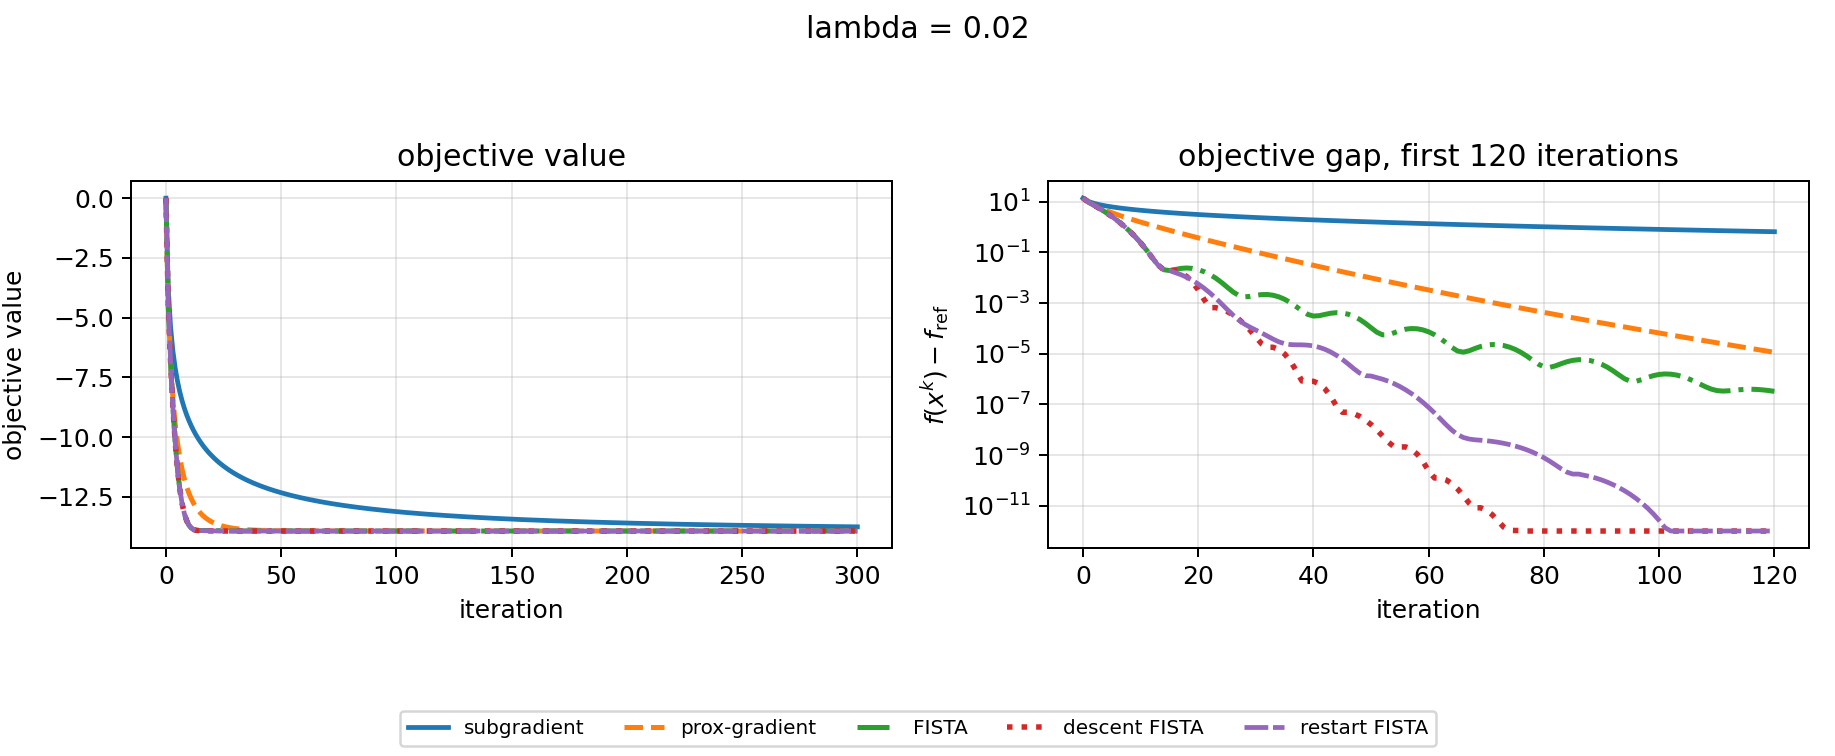
\includegraphics[width=0.96\textwidth]{hw11_lambda_0_02.png}
\end{center}

\begin{center}
  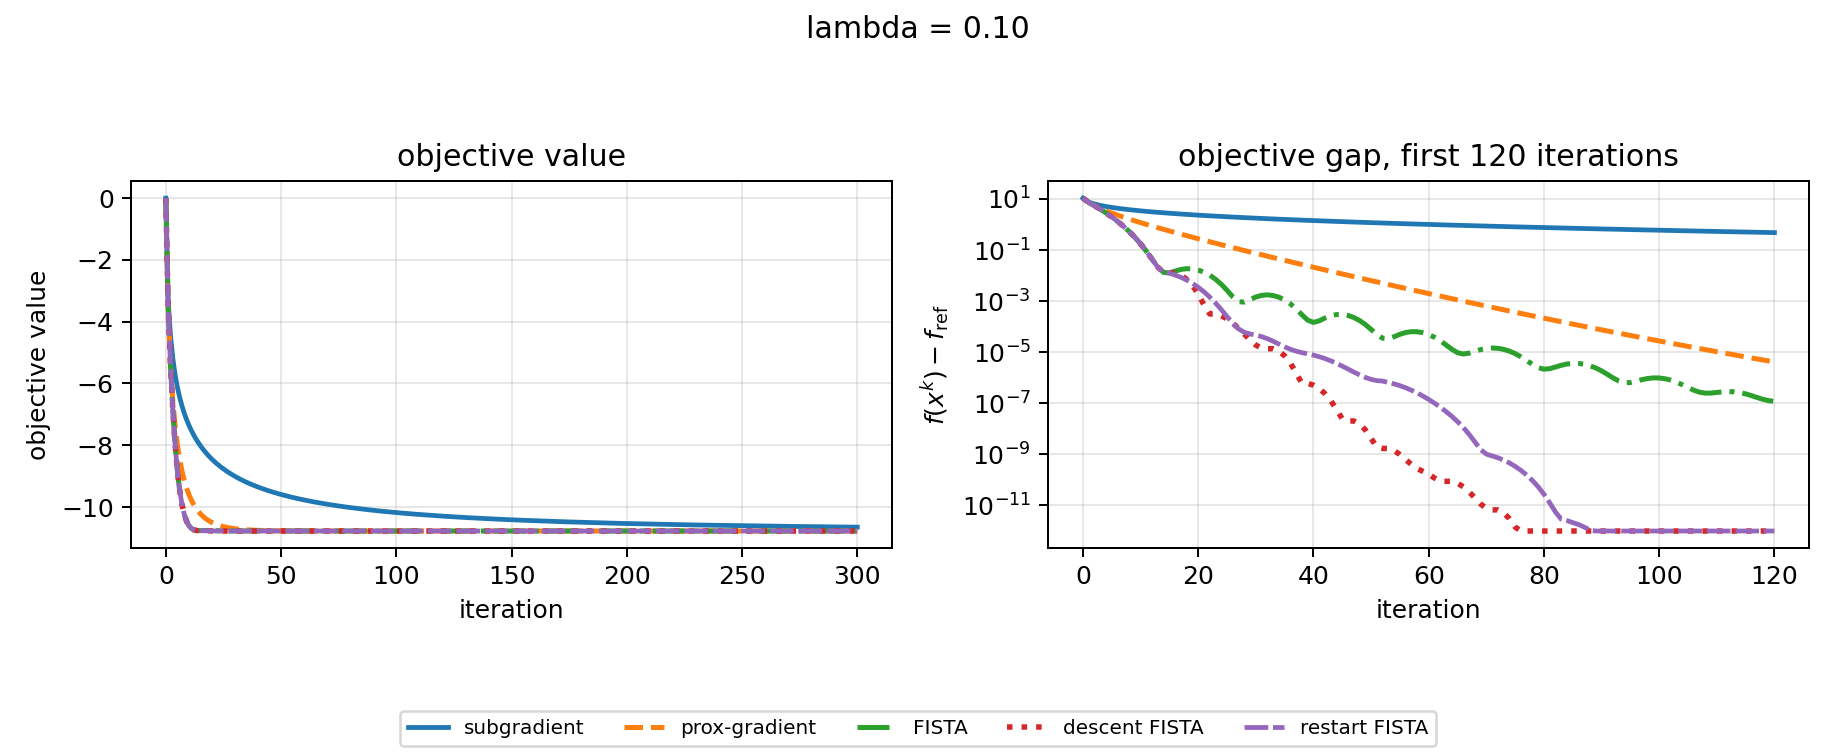
\includegraphics[width=0.96\textwidth]{hw11_lambda_0_10.png}
\end{center}

\begin{center}
  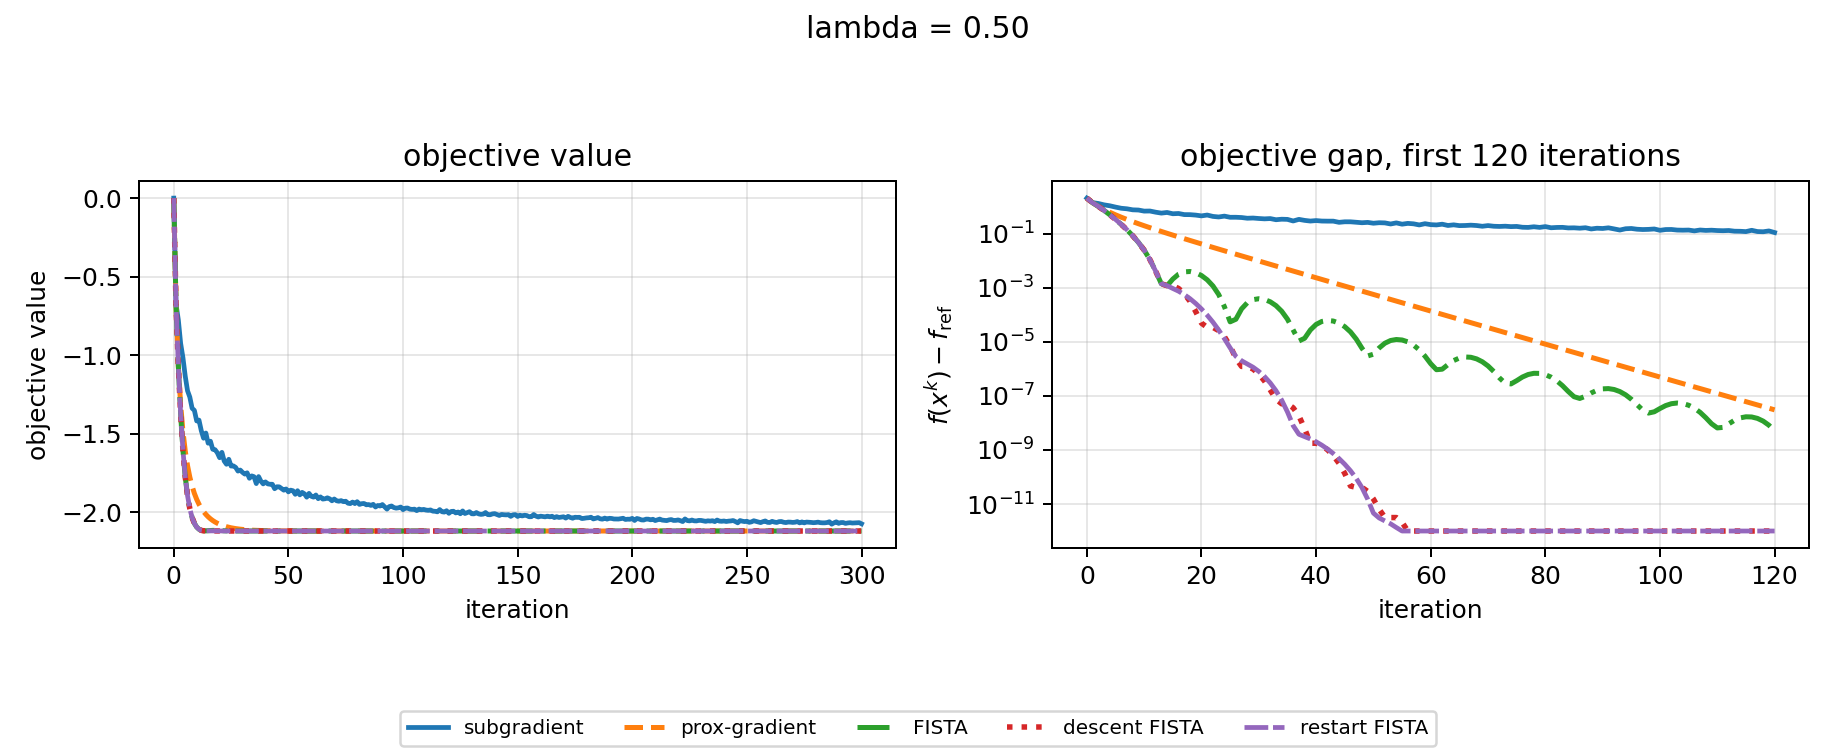
\includegraphics[width=0.96\textwidth]{hw11_lambda_0_50.png}
\end{center}

从图中可以看到，次梯度法下降最慢；近端梯度法稳定下降；FISTA 类方法前期下降更快。右侧半对数图能更明显看出加速方法和普通近端梯度法之间的收敛速度差异。

\appendix
\section{完整代码}
第 2.5 题使用的完整 Python 代码如下。

\lstinputlisting[language=Python]{generate_figures.py}



\end{document}
